% !TEX root = ../../presentation.tex
% Meta: Planung

\begin{slide}{Vision}
  \begin{tikzpicture}[thick, rounded corners=1pt]
    \onslide<2->{
    \draw (0, 0) rectangle ++(5, 2.5)
          node [midway, align=center]
          {\texttt{ERASIM} $\supseteq$ \texttt{Jasmin}};
    }

    \onslide<3->{
    \draw (5.5, 0) rectangle ++(5, 2.5)
          node [midway, align=center] {$|\{\text{Einsatzgebiete}\}| > 1$};
    }

    \onslide<4->{
    \draw (0, -3) rectangle ++(5, 2.5)
          node [midway, align=center]
        {\small \textcolor{Red}{\texttt{0xdead}} $|$ \texttt{addi x1, x0, 42}};
    }

    \onslide<5->{
    \draw (5.5, -3) rectangle ++(5, 2.5);
    \node (arch) at (8, -1.25) {\small\texttt{AbstractArchitecture}};
    \node (x86) at (6.5, -2.25) {\small\texttt{x86}};
    \node (riscv) at (8, -2.25) {\small\texttt{RISC-V}};
    \node (arm) at (9.5, -2.25) {\small\texttt{ARM}};

    \draw [->] (x86) -- (arch);
    \draw [->] (riscv) -- (arch);
    \draw [->] (arm) -- (arch);

    }
  \end{tikzpicture}
\end{slide}

\newlength{\offset}\setlength{\offset}{0.7cm}
\newlength{\step}\setlength{\step}{1.3cm}

\begin{slide}{Planung}
  \begin{tikzpicture}[thick]
    \tikzset{dot/.style={fill, circle, inner sep=1.3pt}};

    % Timeline
    \draw [|->] (0, 0) -- ++(10.5, 0);

    % Timeline Labels
    \foreach \i/\month in {%
      0/Juni, 1/Juli, 2/August, 3/Sept.,%
      4/Oktober, 5/Nov., 6/Dezember, 7/Januar} {
      \draw ({\i * \step + \offset}, 0.125) -- ++(0, -0.25)
            node [below] {\scriptsize\month};
    }

    % Tasks
    \newcommand{\early}{Green}
    \newcommand{\ontime}{ProcessBlue}
    \newcommand{\late}{Red}
    \foreach \name/\month/\y/\dotcolor in {%
      Architektur/0/1/\ontime,%
      Speichermodell/1/2.75/\late,%
      Instruktionen/2.5/0.5/\early,%
      Assemblierung/3.5/2/\late,%
      Direktiven \& Makros/2/4/\late,%
      Serialisierung/4/1/\ontime,%
      Pseudinstruktionen/4/3.5/\ontime,%
      {I/O Module}/5/2.75/\late,%
      Dokumentation/6.5/1.5/\ontime%
    } {
      \path ({\month * \step + \offset}, \y) coordinate [dot, \dotcolor]
            node [above] {\scriptsize\name};
    }

    % Legend
    \path (8.5, 5.5) coordinate [Green, dot] (early)
          node [right] {\scriptsize\hspace{0.1cm}Early};
    \path (early)+(0, -0.4) coordinate [ProcessBlue, dot]
          (ontime) node [right] {\scriptsize\hspace{0.1cm}On Time};
    \path (ontime)+(0, -0.4) coordinate [Red, dot]
          (late) node [right] {\scriptsize\hspace{0.1cm}Late};

    % Legend Bounding Box
    \draw [rounded corners=1pt] (early)+(-0.3, +0.35) rectangle ++(1.6, -1.1);

  \end{tikzpicture}
\end{slide}

\begin{slide}{Planung}
  \begin{tikzpicture}[thick]
    \tikzset{dot/.style={fill, circle, inner sep=1.3pt}};

    % Timeline
    \draw [|->] (0, 0) -- ++(10.5, 0);

    % Timeline Labels
    \foreach \i/\month in {%
      0/Juni, 1/Juli, 2/August, 3/Sept.,%
      4/Oktober, 5/Nov., 6/Dezember, 7/Januar} {
      \draw ({\i * \step + \offset}, 0.125) -- ++(0, -0.25)
            node [below] {\scriptsize\month};
    }

    % Tasks
    \foreach \name/\planned/\actual/\y in {%
      Speichermodell/1/4/2.75,%
      Assemblierung/3.5/6/2,%
      Direktiven und Makros/2/5/4,%
      {I/O Module}/5/7/2.75,
      Instruktionen/2.5/1/0.5%
    } {
      \ifnum\actual<\planned
        \newcommand{\dotcolor}{Green}
      \else
      \newcommand{\dotcolor}{Red}
      \fi
      \path ({\planned * \step + \offset}, \y)
            coordinate [\dotcolor, dot] (p\name);

      \path ({\actual  * \step + \offset}, \y)
            coordinate [\dotcolor, dot] (a\name);

      \draw [->, dotted, \dotcolor]
            (p\name) -- (a\name) node [above, midway]
            {\color{black}\scriptsize\name};
    }

    % Legend
    \path (8.5, 5.5) coordinate [Green, dot] (early)
          node [right] {\scriptsize\hspace{0.1cm}Early};
    \path (early)+(0, -0.4) coordinate [ProcessBlue, dot]
          (ontime) node [right] {\scriptsize\hspace{0.1cm}On Time};
    \path (ontime)+(0, -0.4) coordinate [Red, dot]
          (late) node [right] {\scriptsize\hspace{0.1cm}Late};

    % Legend Bounding Box
    \draw [rounded corners=1pt] (early)+(-0.3, +0.35) rectangle ++(1.6, -1.1);
  \end{tikzpicture}
\end{slide}

% Einige Gruende hierfuer werden im Team Bericht gegeben und diskutiert

\begin{slide}{Exekution}
  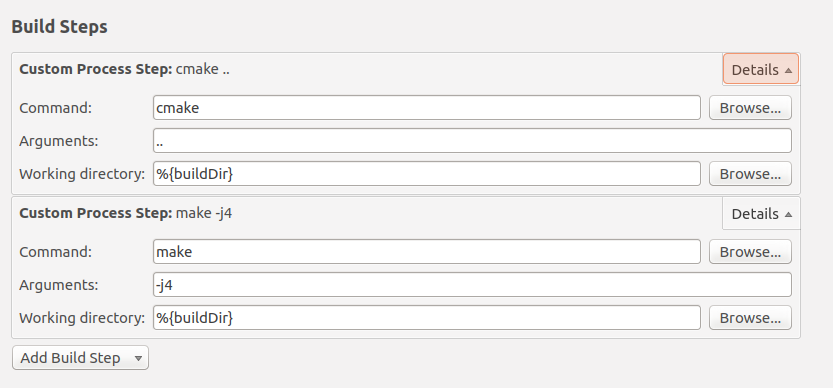
\includegraphics[scale=0.31]{commit-history}
\end{slide}
